\documentclass{article}
\usepackage{graphicx}
\usepackage{authblk}
\usepackage{subcaption}
\usepackage{listings}
\usepackage{booktabs}
\usepackage{biblatex}
\usepackage[utf8]{inputenc}
\usepackage[english]{babel}
\usepackage{csquotes}
\nocite{*}
\addbibresource{report.bib}
\graphicspath{ {./images/} }
\usepackage[a4paper,margin=1in,footskip=0.25in]{geometry}
\begin{document}
    
\title{\textbf{Numerical Simulation Melting of Ice using OpenFOAM}}
\author{Vignesh.S.P\thanks{vikkypandiaraj@gmail.com}}
\affil{M.E. Energy Engineering, College of Engineering Guindy, \\ Anna University.}
\date{}
\maketitle
\begin{abstract}
    This case demonstrates the melting of ice. It’s a example of phase change process. The present case uses a multi-region approach to simulate the phase change process. The simulation is carried out in OpenFOAM v1906 using the solver \textbf{chtMultiRegionFoam} and the phase change is handled by \textbf{solidficationMeltingSource} source term. The geometry is a 2-D pipe and the flow is laminar and transient. The volume fraction of melting water is obtained from the simulation and is analyzed. 
\end{abstract}

    

\section{Introduction}
    \paragraph*{}
    The purpose of this case is to simulate the phase change process of melting of ice inside a cylindrical pipe. This case study introduces \textbf{solidficationMeltingSource} source term which governs the mushy phase change process. The simulation is carried out in OpenFOAM v1906. The solver employed here is \textbf{chtMultiRegionFoam} a conjugate heat transfer solver with coupled heat transfer between solid and fluid.


\section{Case Setup}
    \subsection{Geomety}
    \paragraph*{}
    This case considers the transient simulation of conjugate heat transfer. Figure 1.a shows the dimensions of geometry considered in study. The geometry is a 2 dimensional case of a copper cylindrical pipe  of outer diameter of 30 mm and thickness of 5mm with infinite dimension along Z direction. The geometry  is made of blocks  to aid hexahedral meshing as seen in Figure \ref{fig:Geometry}. The geometry is modelled and meshed in Salome-Meca.
    
    \begin{figure}[ht]
        \centering
        \begin{subfigure}[b]{0.4\linewidth}
            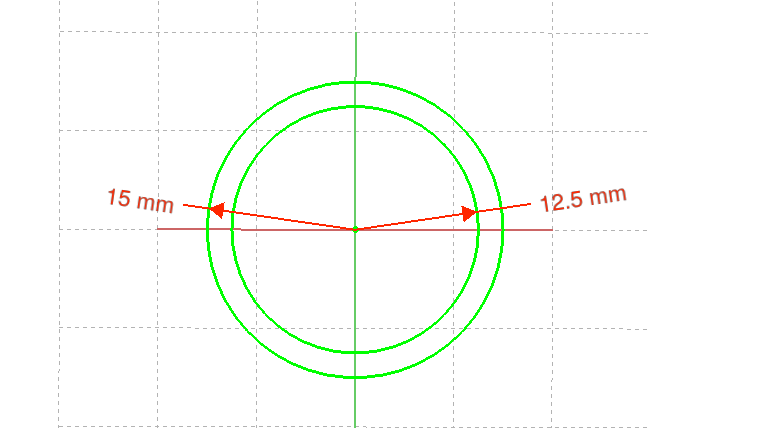
\includegraphics[width=\linewidth]{drawing.png}
            \caption{Geometry}
        \end{subfigure}
        \begin{subfigure}[b]{0.4\linewidth}
            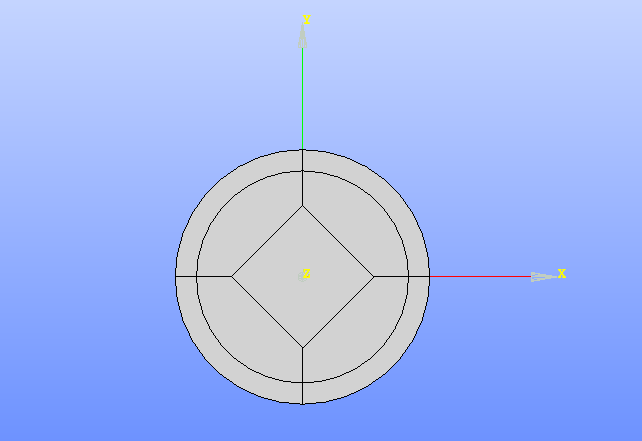
\includegraphics[width=\linewidth]{geometry.png}
            \caption{Geometry with blocks}
        \end{subfigure}
        \caption{Geometry of the Computational Domain}
        \label{fig:Geometry}
    \end{figure}

    \subsection{Mesh}
    \paragraph*{}
    The mesh is created using Salome-Meca hexahedral mesher. The patches are named as well the zones are also names as solidZone and fluidZone and the mesh is exported as UNV file from Salome-Meca. The \textbf{ideasUnvToFoam} utility is used to import the mesh into OpenFOAM case. Using \textbf{splitMeshRegions} utility the mesh is seperated into fluid region and solid region from the named zones. The meshes of both solid region and fluid region are listed in Figure \ref{fig:Mesh}. The solid region has a cell count of 3600 and the fluid region has a cell count of 4500.
    
    \begin{figure}[ht]
        \centering
        \begin{subfigure}[b]{0.4\linewidth}
            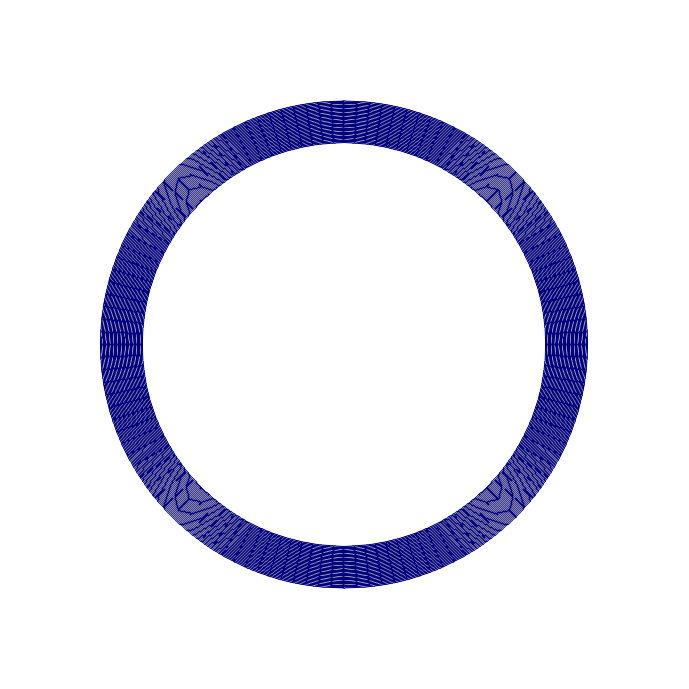
\includegraphics[width=\linewidth]{solidzone.png}
            \caption{Solid region Mesh}
        \end{subfigure}
        \begin{subfigure}[b]{0.4\linewidth}
            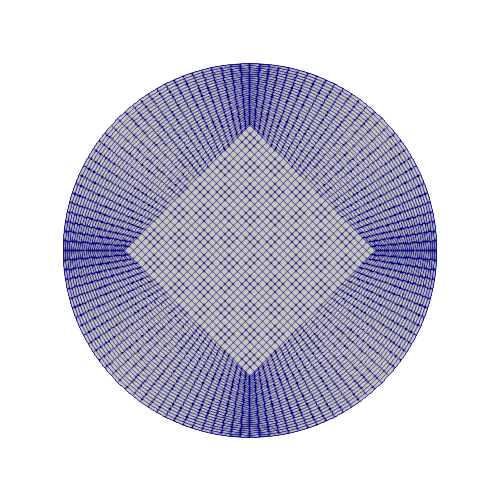
\includegraphics[width=\linewidth]{fluidzone.png}
            \caption{Fluid region Mesh}
        \end{subfigure}
        \caption{Computational Mesh}
        \label{fig:Mesh}
    \end{figure}

    \subsection{Boundary Conditions}
    \paragraph*{}
    The initial and boundary condition for patches are specified as in 0/ directory. The solid and fluid zones have a coupled patch through which the temperature is transported. The outer walls of solid region is maintained at a constant temperature of 298 K. The boundary Conditions are lised in table \ref{tab:fluidbc} and table \ref{tab:solidbc} for fluid and solid regions respectively.

    \begin{table}[ht]
        \centering
        \begin{tabular}{@{}lll@{}}
        \toprule
        Boundary & fluidFrontAndBack & fluidZone\_to\_solidZone \\ \midrule
        p & empty & calculated \\
        p\_rgh & empty & fixedFluxPressure \\
        T & empty & compressible::turbulentTemperatureCoupledBaffleMixed \\
        U & empty & noSlip \\
        fluidZone:alpha1 & empty & zeroGradient \\
        cellToRegion & zeroGradient & calculated \\ \bottomrule
        \end{tabular}
        \caption{Fluid Boundary Conditions}
        \label{tab:fluidbc}
    \end{table}

    \begin{table}[h]
        \centering
        \begin{tabular}{@{}lll@{}}
        \toprule
        Boundary & solidWall & solidZone\_to\_fluidZone \\ \midrule
        p & calculated & calculated \\
        T & fixedValue & compressible::turbulentTemperatureCoupledBaffleMixed \\
        cellToRegion & zeroGradient & calculated \\ \bottomrule
        \end{tabular}
        \caption{Solid Boundary Conditions}
        \label{tab:solidbc}
    \end{table}

    \subsection{Melting Source}
    \paragraph*{}
    The source terms which governs the melting of ice is \textbf{solidficationMeltingSource} which is enabled by using fvOptions utility. This source is designed to model the effect of solidification and melting processes, e.g. windshield defrosting.  The phase change occurs at the melting temperature, \textbf{Tmelt}. The presence of the \textbf{solid phase} in the flow field is incorporated into the model as a \textbf{momentum porosity} contribution; the \textbf{energy} associated with the phase change is added as an \textbf{enthalpy} contribution. The model generates a field "zoneName:alpha1" which can be visualised to to show the melt distribution as a fraction with values ranging from 0 to 1. The details to be enterend in the fvOptions file is as follows

    \begin{lstlisting}
    fluidZone //name of the zone
    {
        type            solidificationMeltingSource;
        active          on;
        solidificationMeltingSourceCoeffs
        {
            selectionMode   all;    // Cell selection mode 
            Tmelt           273;    // Saturation temperature [K]
            L               334000; // Enthalpy of fusion for water [J/kg]
            thermoMode      thermo; // Retrieve thermo properties 
            beta            50e-6;  // Thermal expansion coeff [1/K]
            rhoRef          916.8;  // Reference Solid Density [kg/m^3]
        }
    }
        
    \end{lstlisting}

    \section{Result and Discussion}
    \paragraph*{}
    The simulation carried out with adjustable run time which adjusts the time step in  accordance to Courant Number. After the simulation is done post processing is done. 
    
    \subsection{Post Processing}
    \paragraph*{}
    The post processing is done using \textbf{paraview} software. The Scalar field \textsl{alpha1} is visualised to understand the melting of ice along with velocity \textsl{U} and temperature \textsl{T}. The command \textbf{paraFoam -touch-all} is used to read all the data from all regions then paraview is opened up and the file \textbf{postProcess.pvsm} loaded up for visualizing the results.

    \subsection{Results}
    \paragraph*{}
    From the Figure \ref{fig:res0-1000}, the melting front is being visualised on the left for time from 10s to 1000s, in which the black coloured contour region represents the fluid phase and the gray colour represents the solid phase. There is no velocity in the solid phase as the solver ignores the cells with \textsl{alpha1} = 0 since while solving momentum equation. The melting front start fast adnd slows down as more solid phase melts into fluid. 
    
    \paragraph*{}
    From the Figure \ref{fig:resFinal}, the melting of solid takes place at a very slow phase, the solid phase takes a time of 2870 s to completely melt. After which the simulation changes to natural convection of the melted fluid.
    \begin{figure}[ht]
        \centering
        
        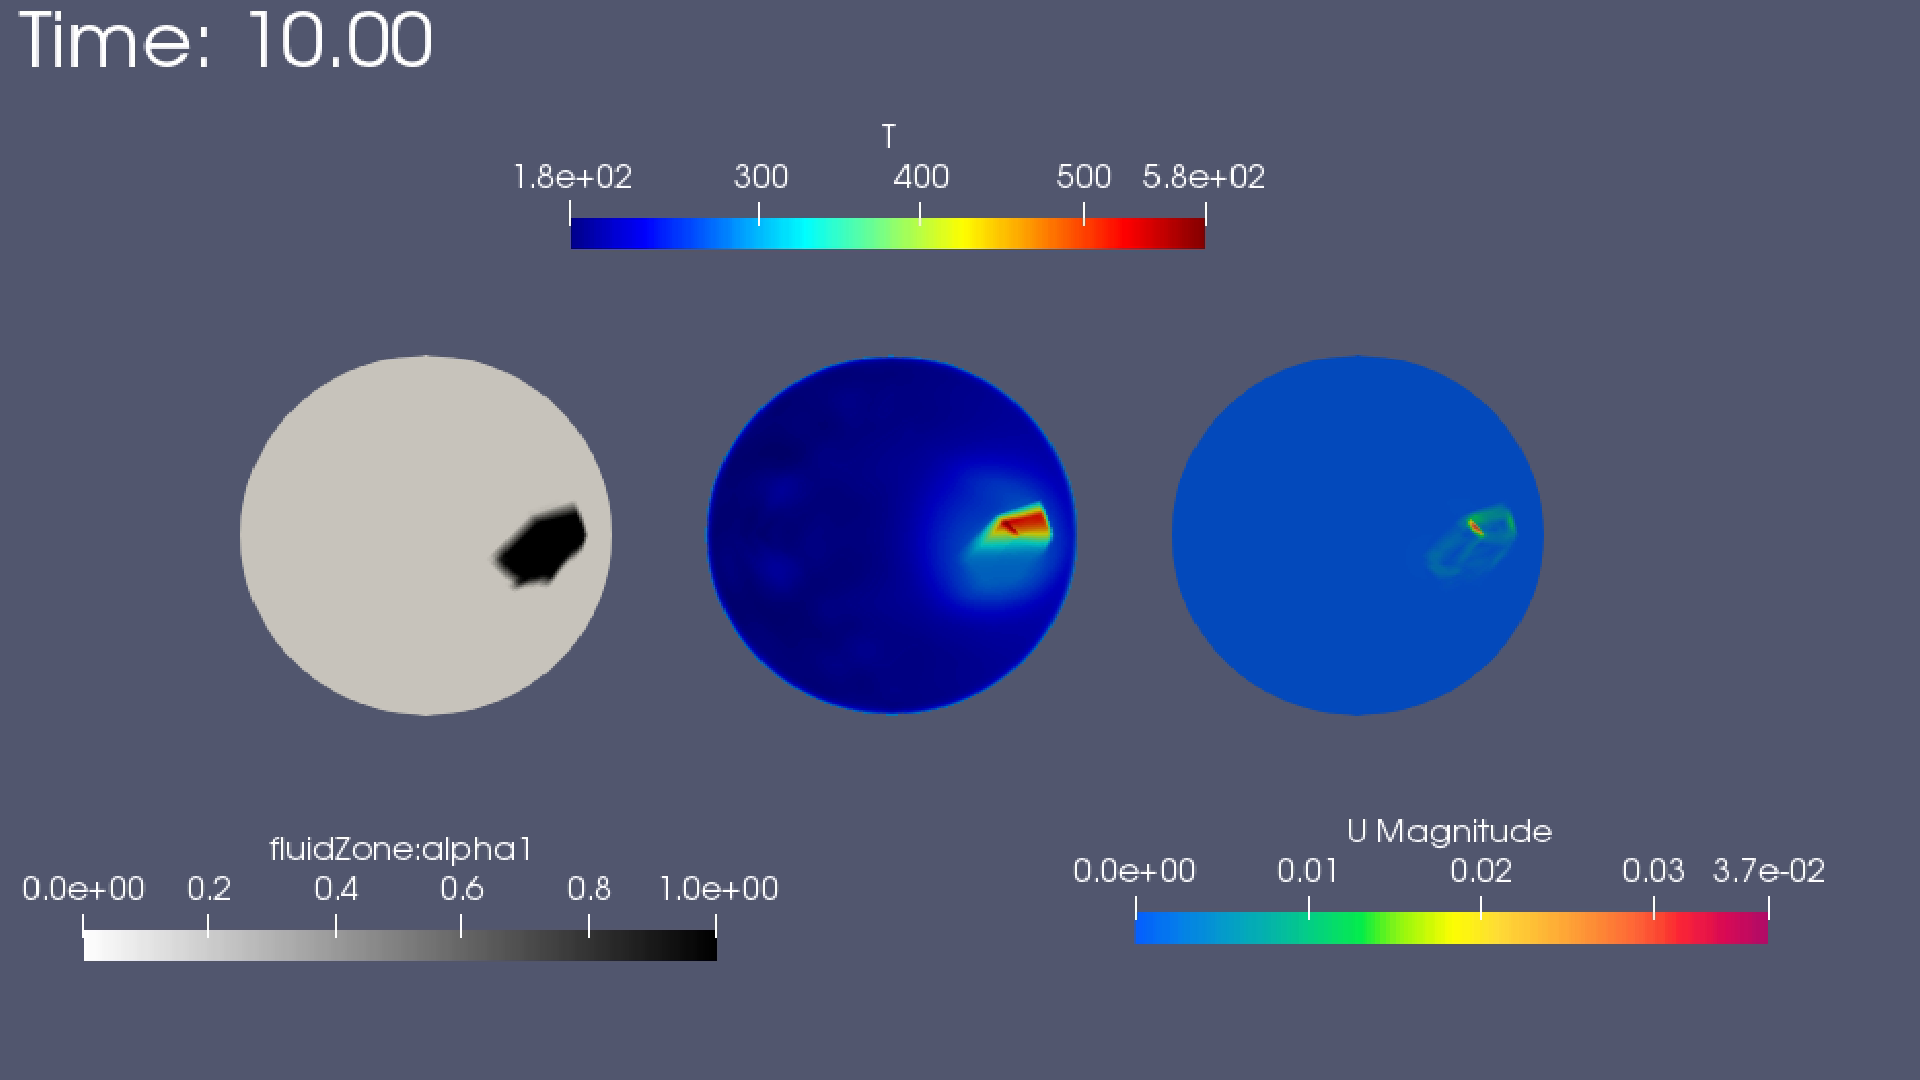
\includegraphics[width=0.65\linewidth]{time10.png}
        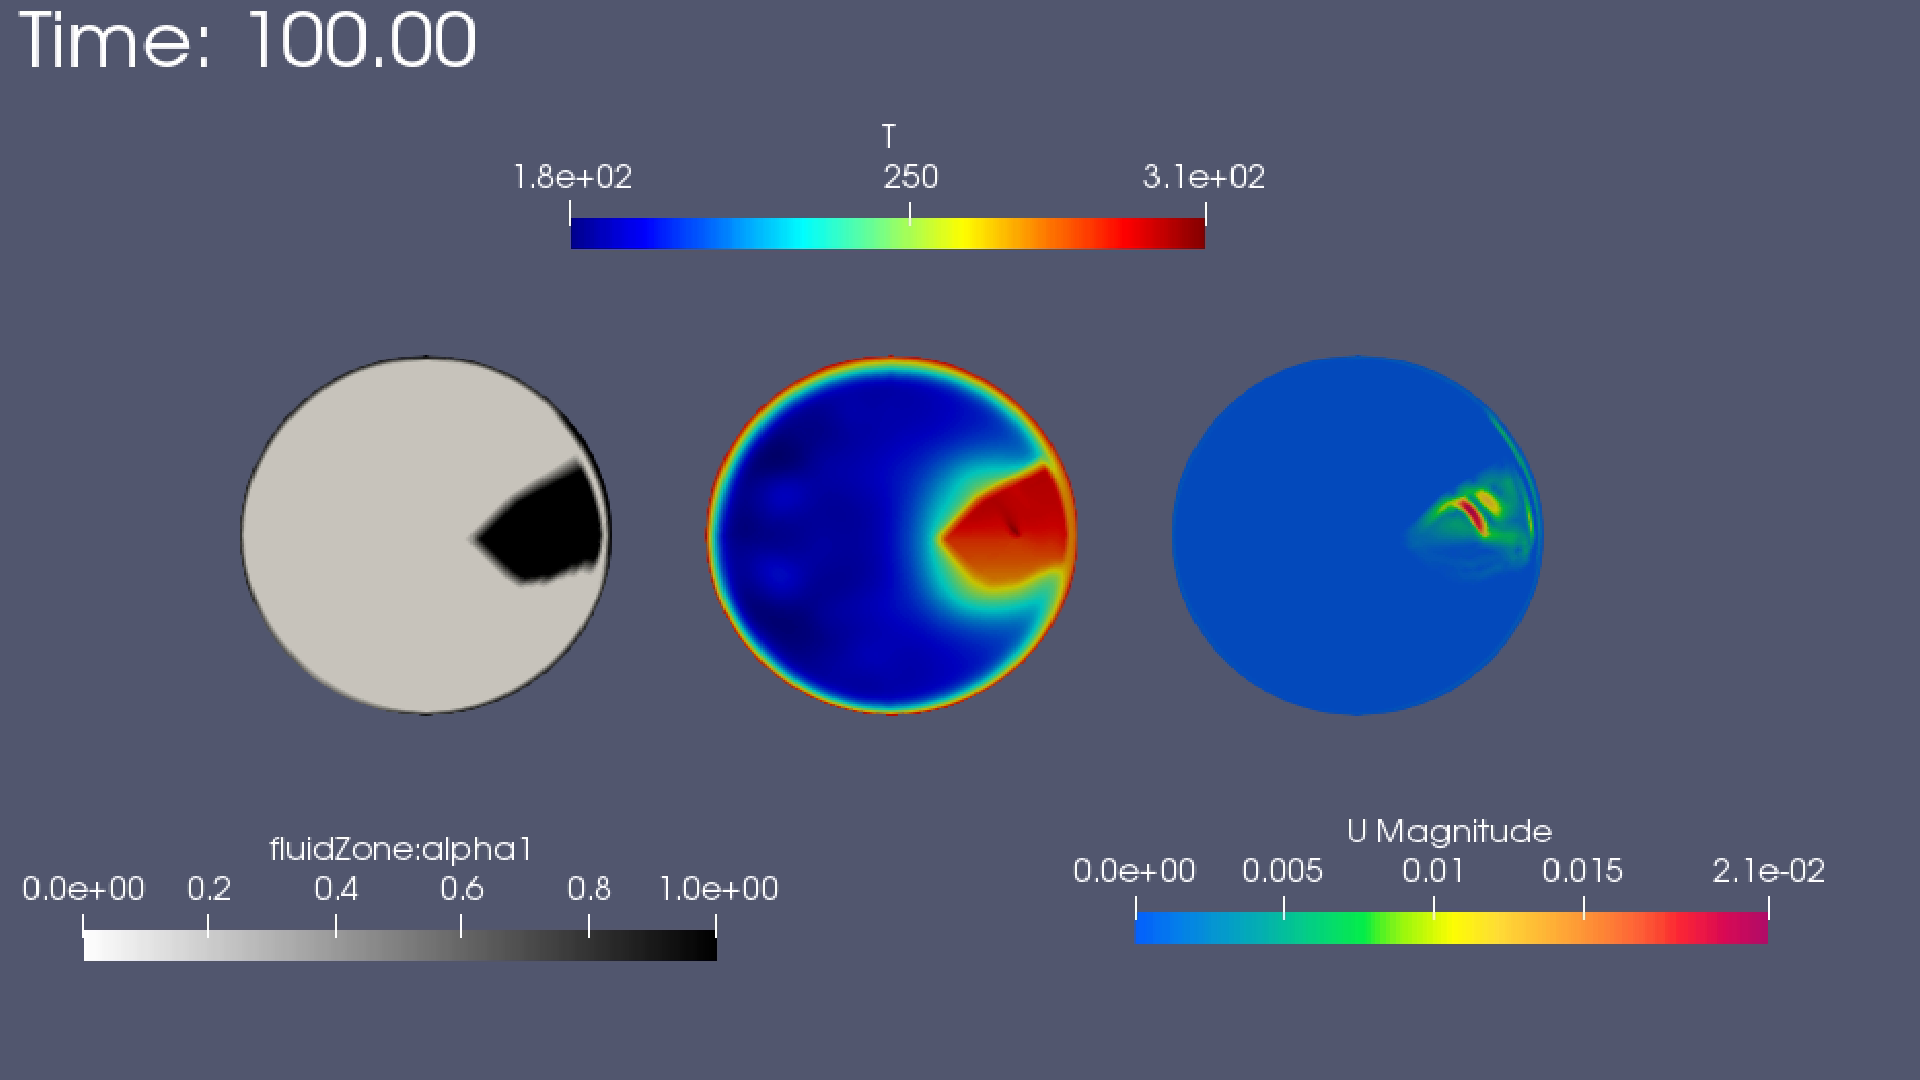
\includegraphics[width=0.65\linewidth]{time100.png}
        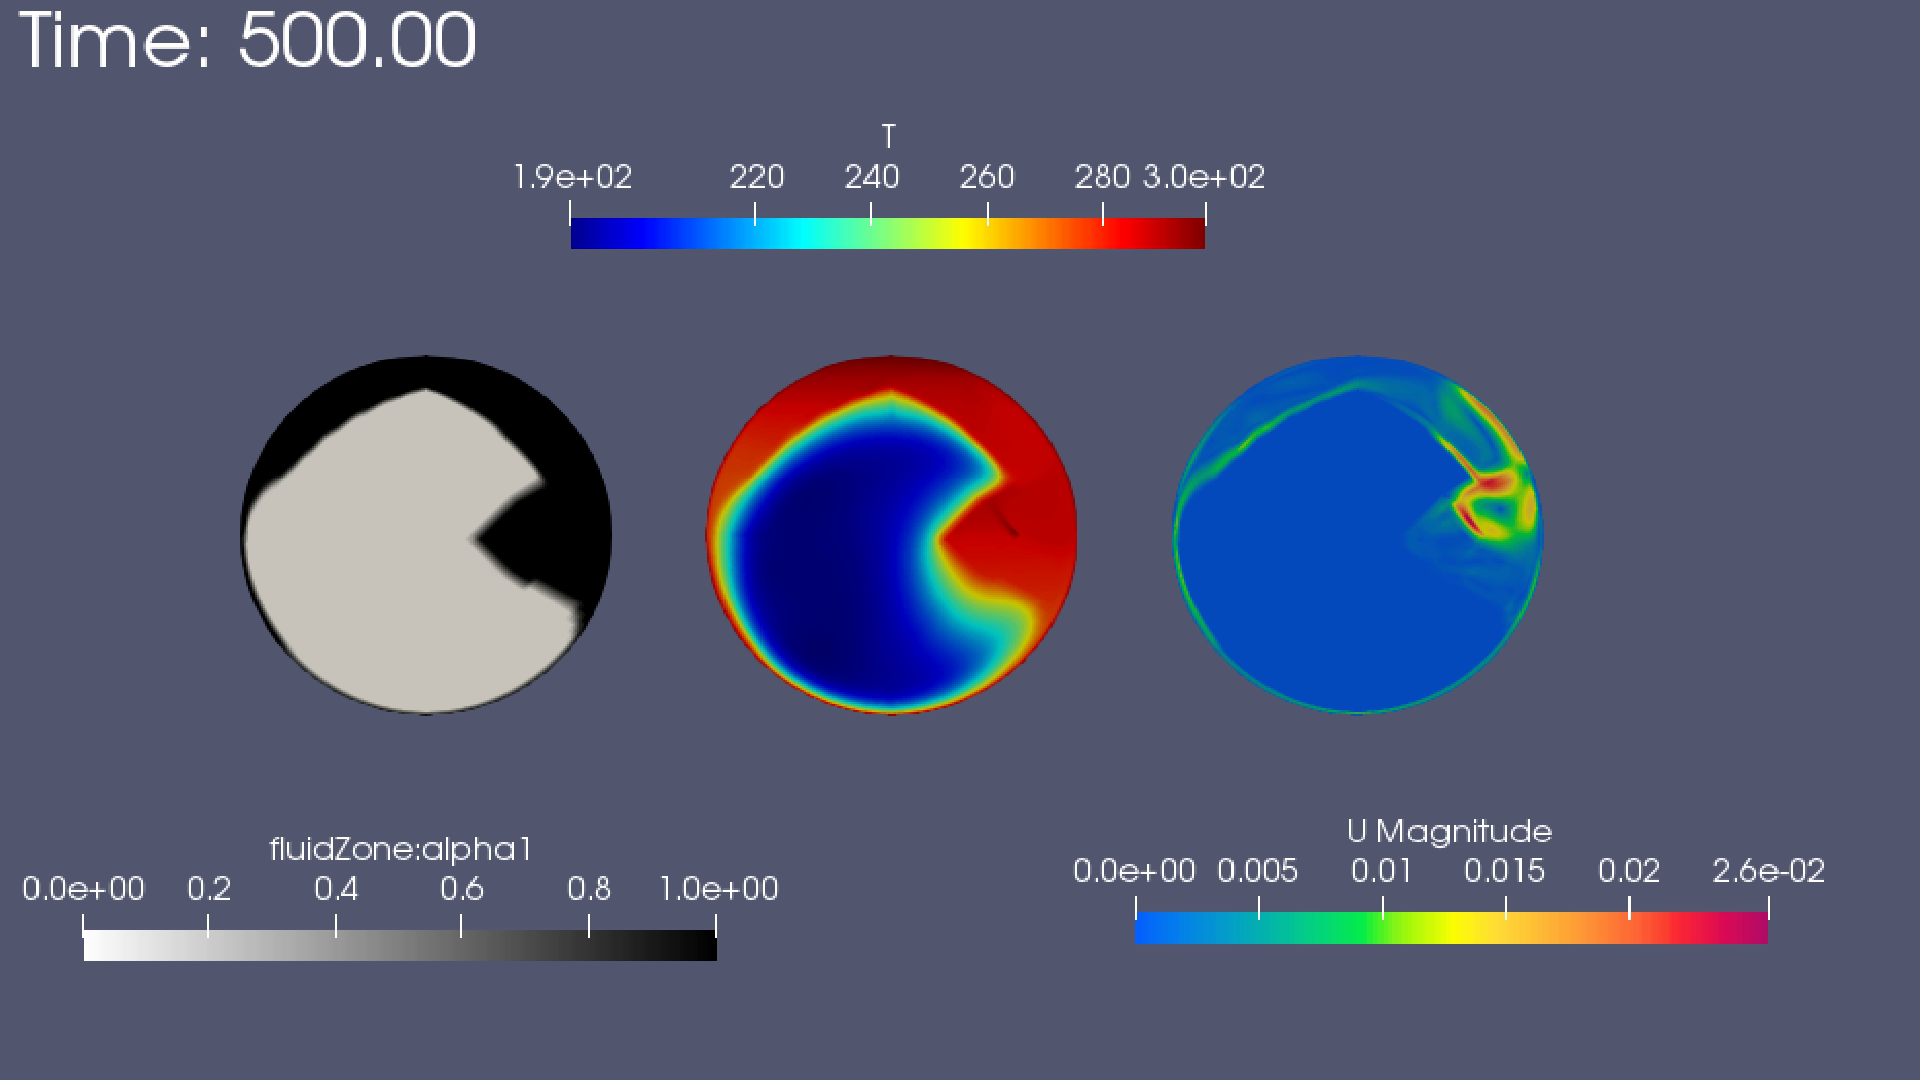
\includegraphics[width=0.65\linewidth]{time500.png}
        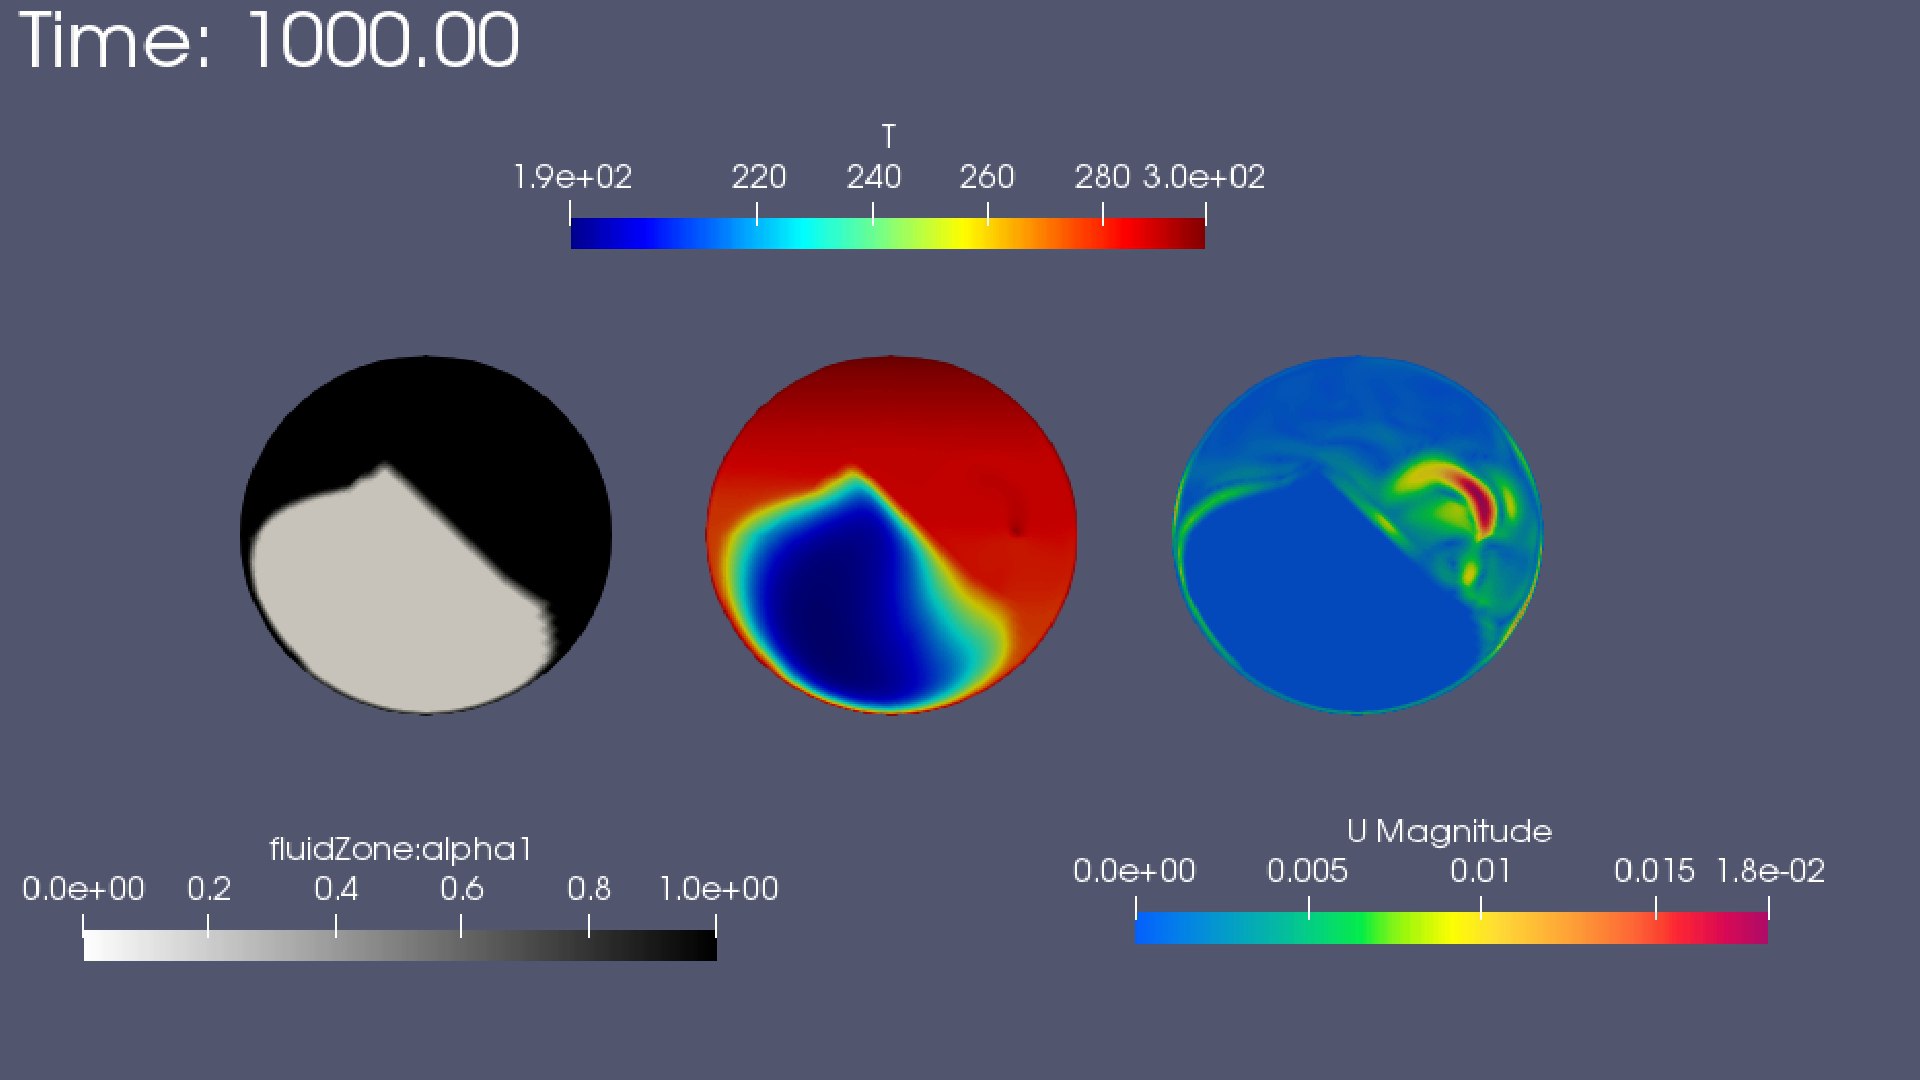
\includegraphics[width=0.65\linewidth]{time1000.png}
        \caption{Contour plots of \textsl{alpha1, T, U}} at different time steps
        \label{fig:res0-1000}
    \end{figure}
    
    \begin{figure}[ht]
        \centering
        
        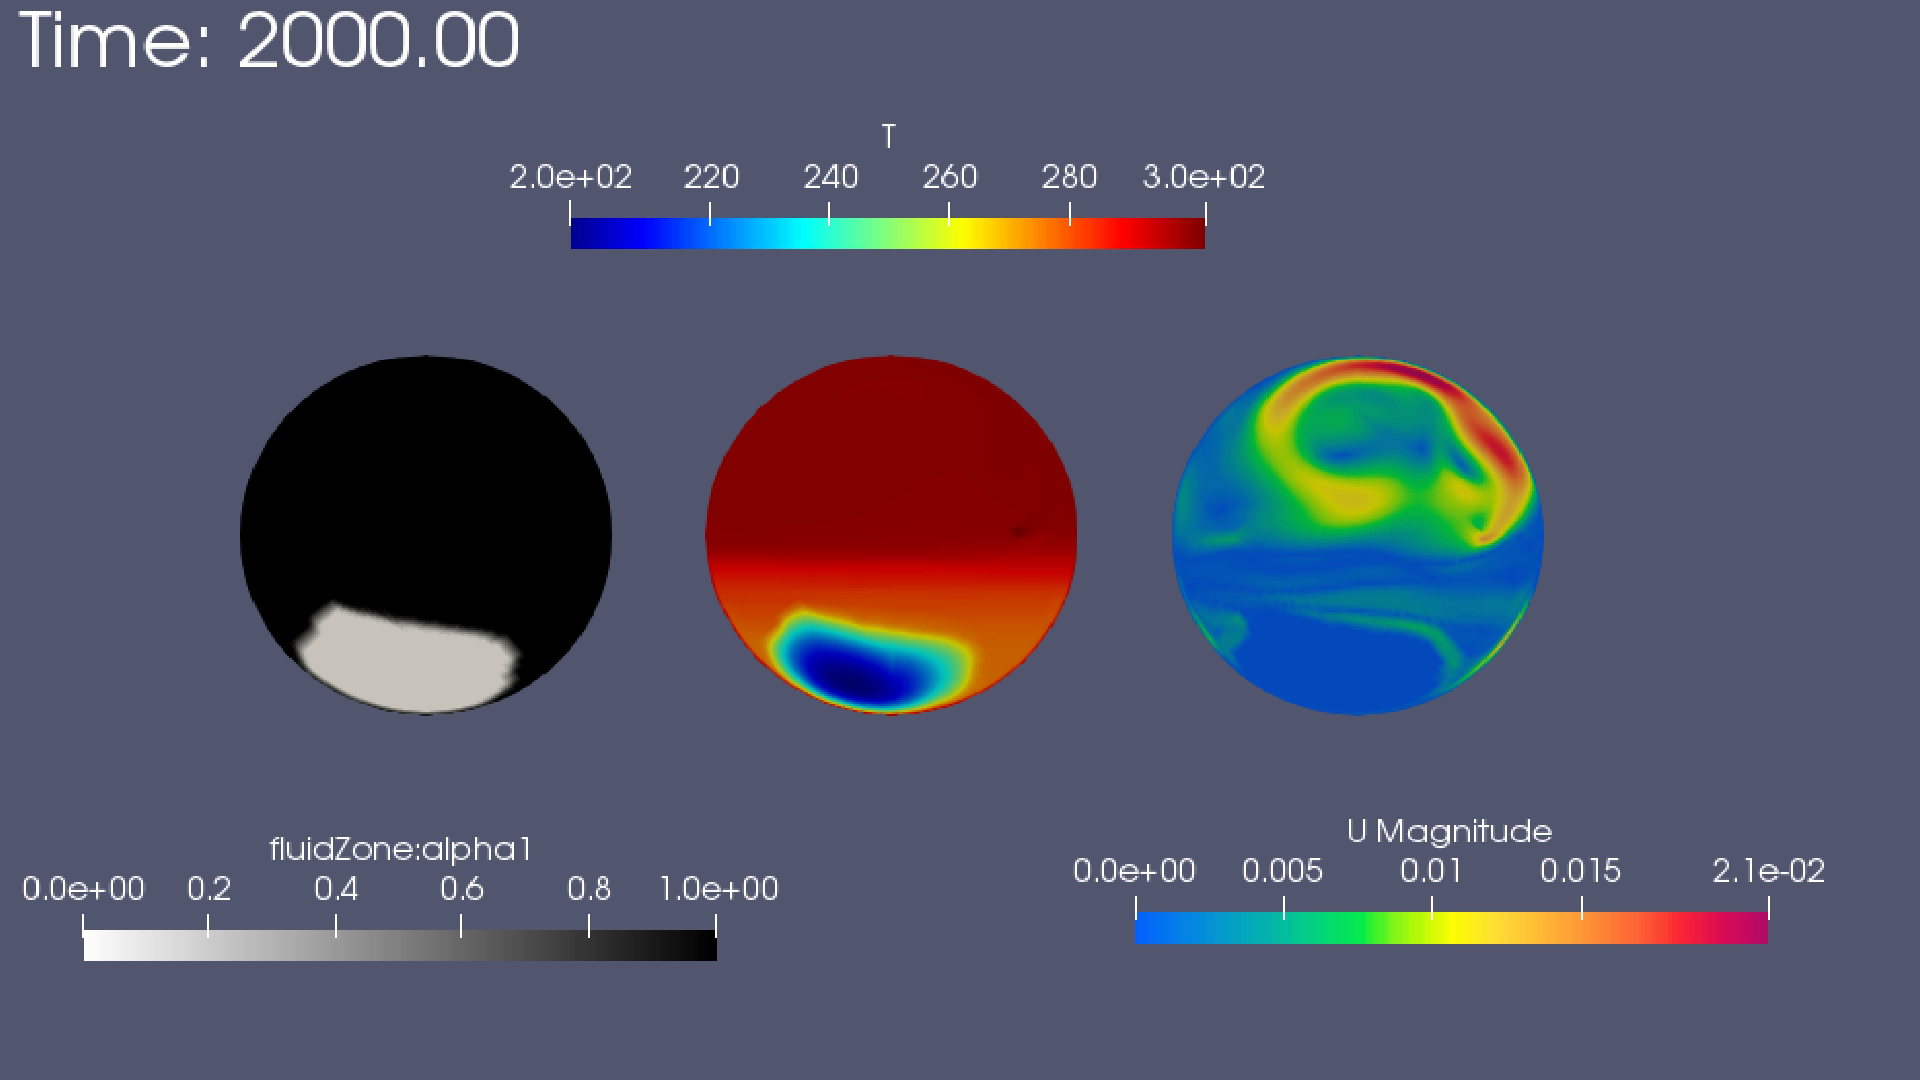
\includegraphics[width=0.75\linewidth]{time2000.png}
        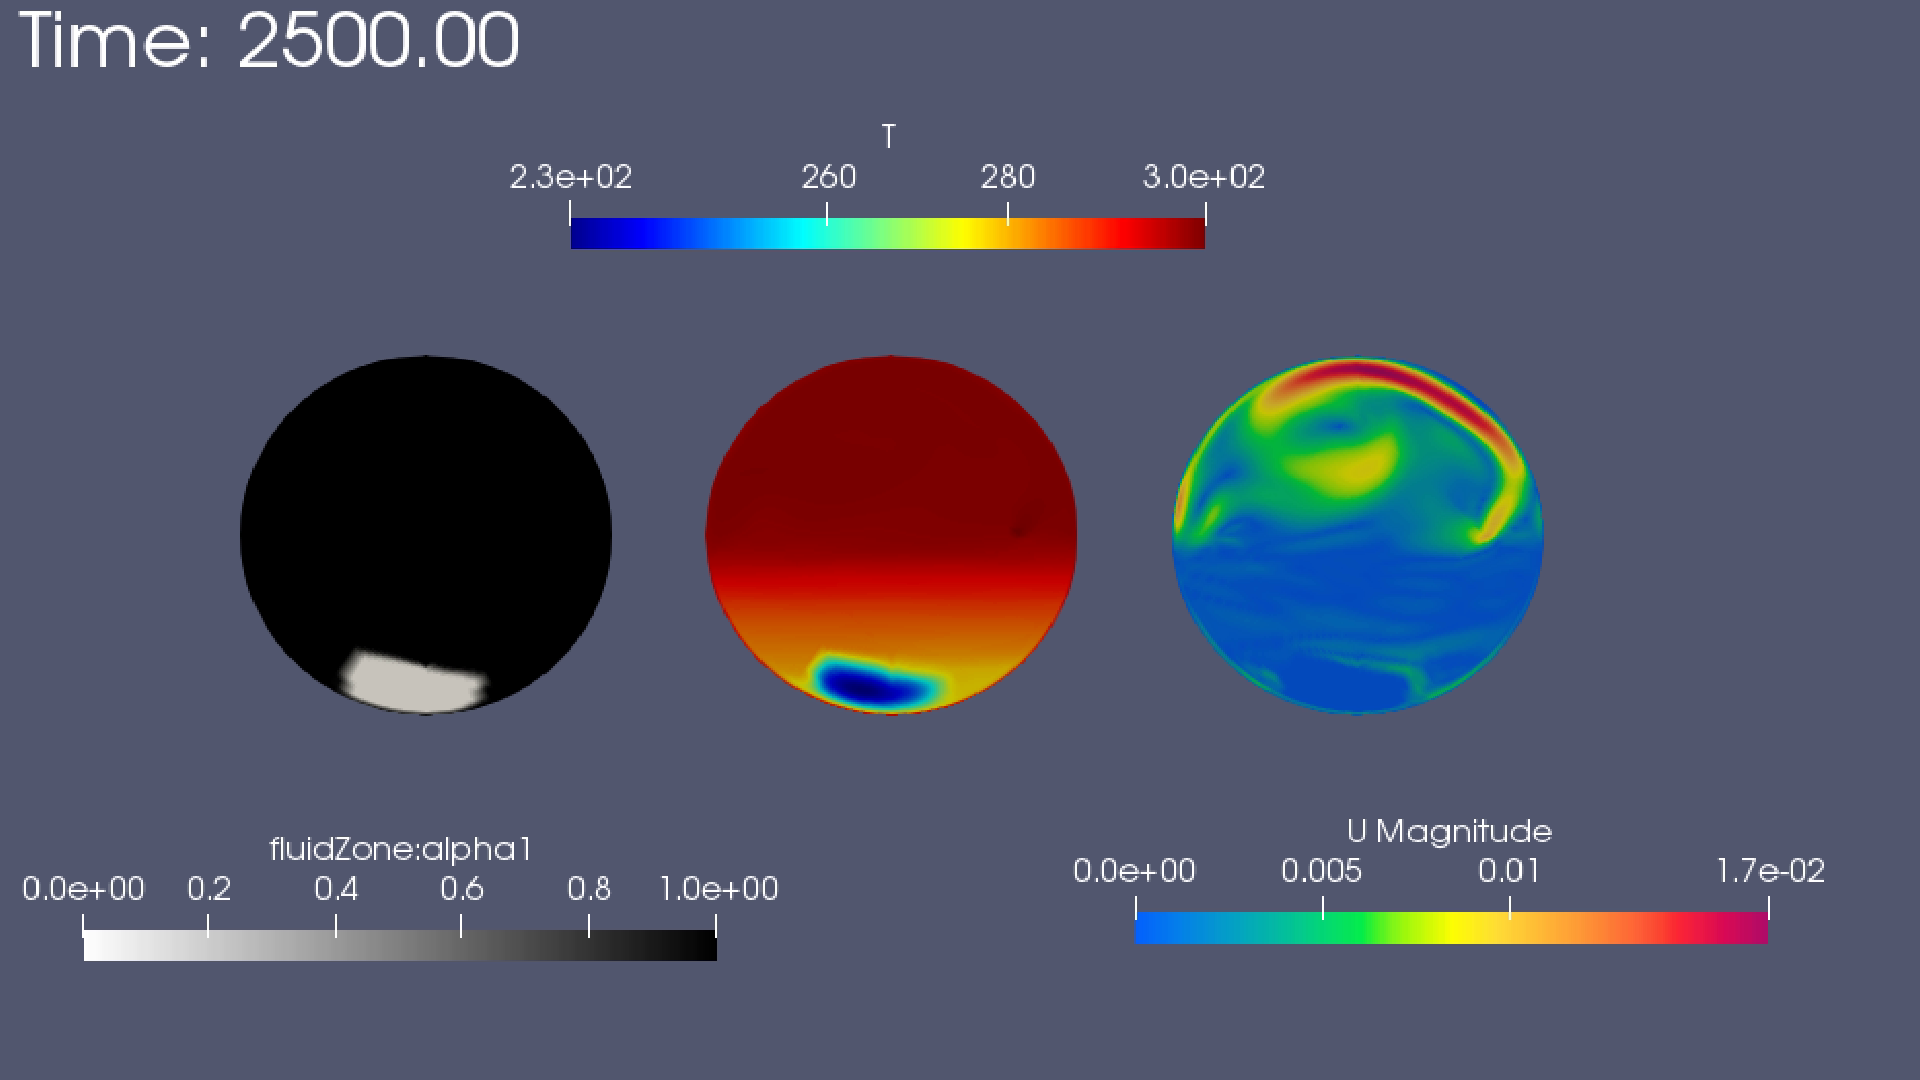
\includegraphics[width=0.75\linewidth]{time2500.png}
        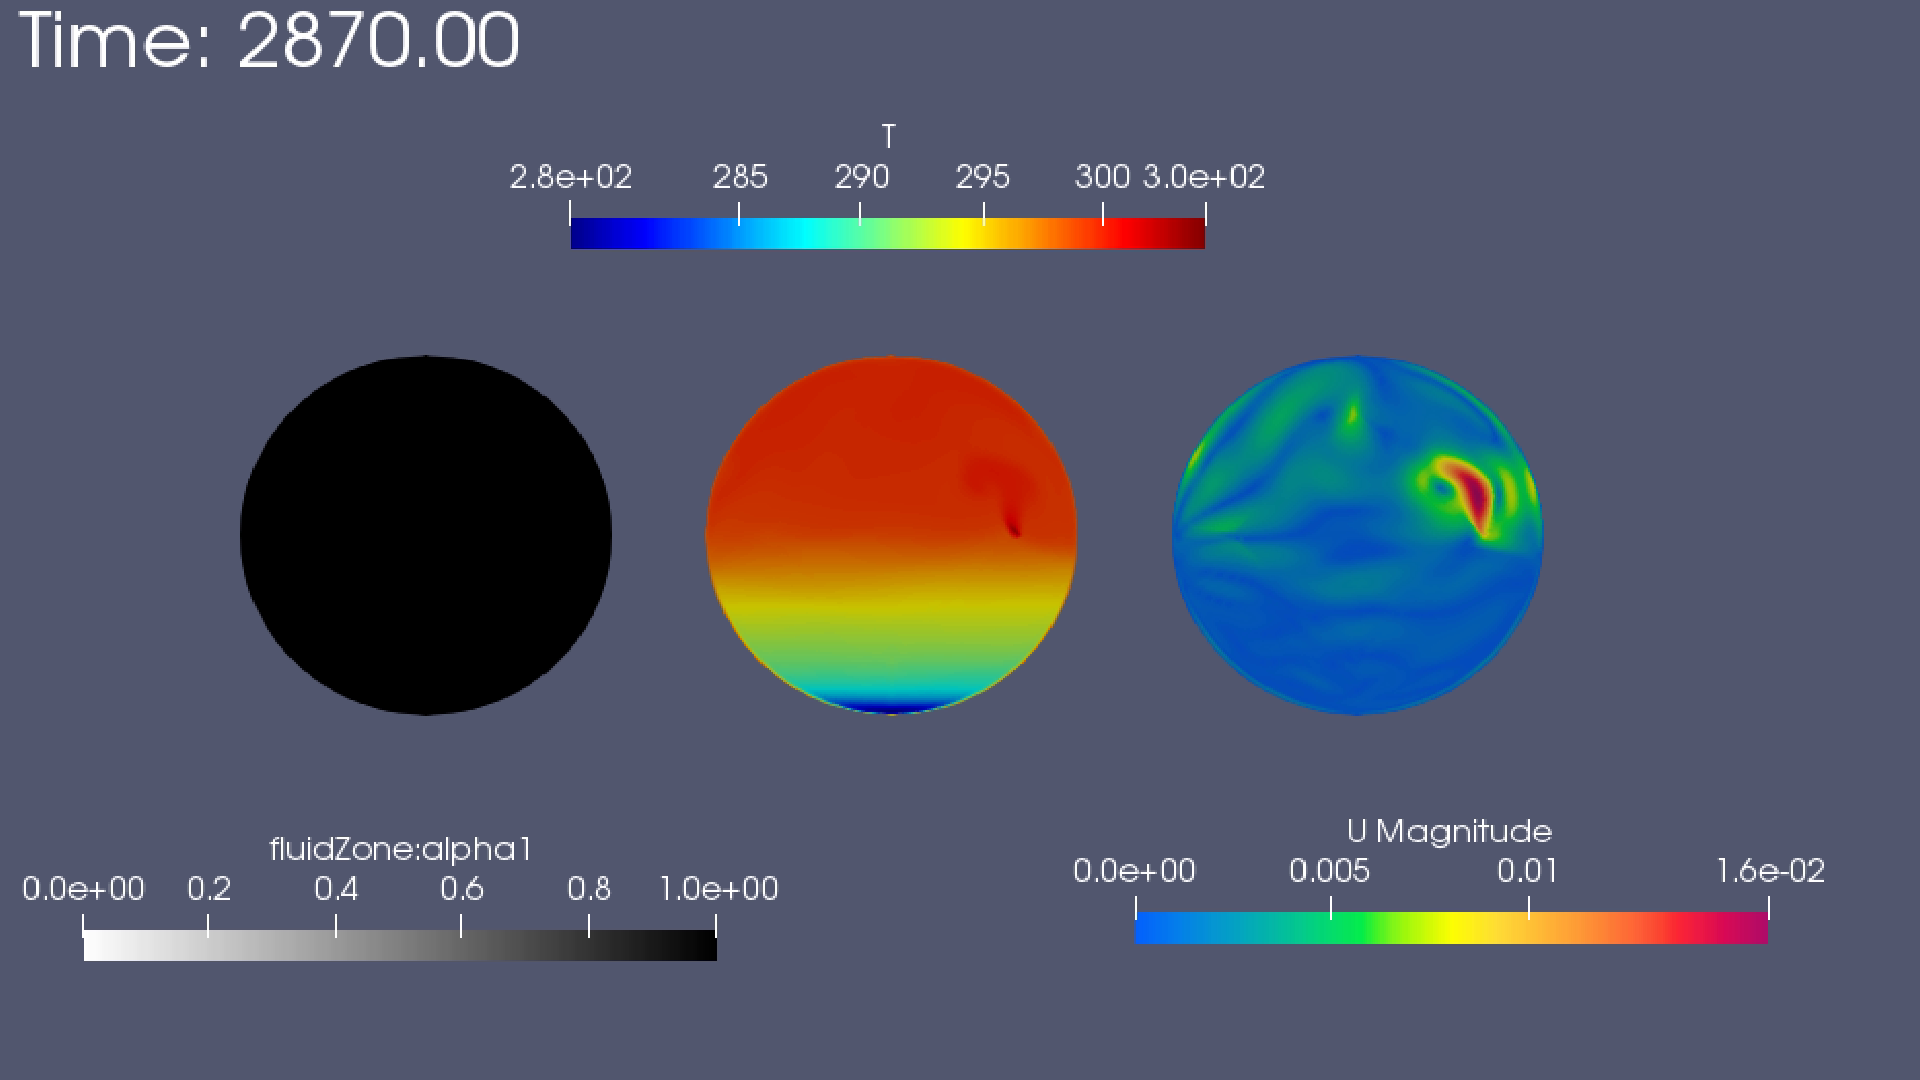
\includegraphics[width=0.75\linewidth]{time2870.png}
        \caption{Contour plots of \textsl{alpha1, T, U}} at time 2000 s, 2500 s and 2870 s. 
        \label{fig:resFinal}
    \end{figure}
    \clearpage
    \printbibliography

\end{document}
